%-------------------------------------------------------------------------------
% SECTION TITLE
%-------------------------------------------------------------------------------

\cvsection{Publications}


%-------------------------------------------------------------------------------
% CONTENT
%-------------------------------------------------------------------------------
% \item \cvpub{\textbf{\bodyfontlight Large Language Models Show Human-like Social Desirability Biases in Survey Responses\\ } \textbf{\bodyfontlight{Aadesh Salecha}}, Molly Ireland, Shashanka Subrahmanya, João Sedoc, Lyle Ungar, and Johannes Eichstaedt. \emph{Proceedings of the National Academy of Sciences (PNAS Nexus)} \href{https://www.arxiv.org/abs/2405.06058}{\textcolor{MidnightBlue}{arxiv.org/abs/2405.06058}} \\
% (accepted; pending revisions)}

%---------------------------------------------------------
% \cvsubsection{Published}
%---------------------------------------------------------

\cvsubsection{Highlights}

\begin{center}
% --- Left: Bar Chart in a minipage ---
\begin{minipage}[t]{0.55\textwidth}
    \centering
    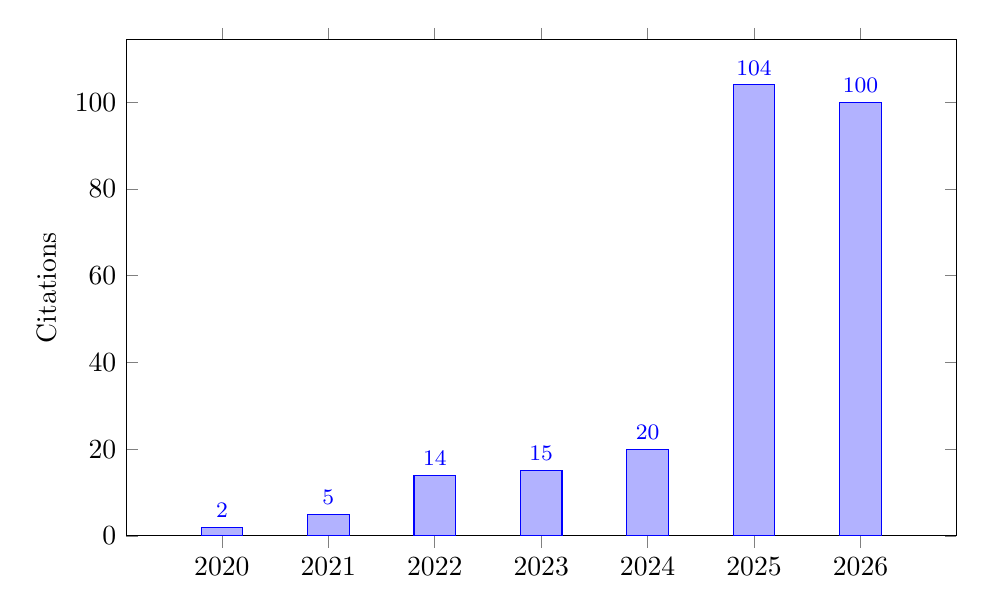
\begin{tikzpicture}
    \begin{axis}[
        ybar,
        bar width=15pt,
        ymin=0,
        ylabel={Citations},
        xtick=data,
        enlarge x limits=0.15,
        nodes near coords,
        every node near coord/.append style={font=\footnotesize},
        width=\linewidth,
        height=0.65\linewidth,
% AUTOGEN:CHART:START
        symbolic x coords={2020,2021,2022,2023,2024,2025,2026},
    ]
    \addplot coordinates {(2020,2) (2021,5) (2022,14) (2023,15) (2024,20) (2025,104) (2026, 100)};
% AUTOGEN:CHART:END
    \end{axis}
    \end{tikzpicture}
\end{minipage}
\hfill
% --- Right: Metrics Table in a minipage ---
\begin{minipage}[t]{0.4\textwidth}
    \vspace{-100pt}
    \begin{tabular}{@{}ll@{}}
% AUTOGEN:METRICS:START
        \textbf{\bodyfontlight Total Publications:}       &  16  \\
        \textbf{\bodyfontlight Total citations:} & 178 \\
        \textbf{\bodyfontlight h-index:}         & 6  \\
% AUTOGEN:METRICS:END
    \end{tabular}
\end{minipage}
\end{center}



\begin{enumerate}
\label{sec:llmpsych}

  \item \cvpub{\textbf{\bodyfontlight Large Language Models Display Human-like Social Desirability Biases in Big Five Personality Surveys\\} \textbf{\bodyfontlight{Aadesh Salecha}}, Molly E. Ireland, Shashanka Subrahmanya, João Sedoc, Lyle H. Ungar, and Johannes C. Eichstaedt. \emph{PNAS Nexus}, Vol. 3, No. 12, pg. e533, 2024. \href{https://doi.org/10.1093/pnasnexus/pgae533}{\textcolor{MidnightBlue}{academic.oup.com/pnasnexus/article/3/12/pgae533/7919163}}}
   \href{https://www.wired.com/story/chatbots-like-the-rest-of-us-just-want-to-be-loved/}{\textcolor{MidnightBlue}{WIRED Magazine Article: Chatbots, Like the Rest of Us, Just Want to Be Loved}}

\end{enumerate}

\cvsubsection{Journal Publications}
\begin{enumerate}
\setcounter{enumi}{1}

\label{sec:adampnas}
\item \cvpub{\textbf{\bodyfontlight Monitoring the Opioid Epidemic via Social Media Discussions.\\ } Adam Lavertu, Tymor Hamamsy, \textbf{\bodyfontlight{Aadesh Salecha}}, Delaney Smith, Johannes Eichstaedt, and Russ B Altman. \emph{Nature Partner Journals: Digital Medicine.} \href{https://www.nature.com/articles/s41746-025-01642-x}{\textcolor{MidnightBlue}{nature.com/articles/s41746-025-01642-x}}}

\label{sec:fakenewsjournal}
\item \cvpub{\textbf{\bodyfontlight Fake News Spreader Detection using Trust-based strategies in Social Networks with Bot Filtration.\\ } Bhavtosh Rath, \textbf{\bodyfontlight{Aadesh Salecha}}, and Jaideep Srivastava. \emph{Social Network Analysis and Mining (SNAM)} (2022)\\\href{https://doi.org/10.1007/s13278-022-00890-z}{\textcolor{MidnightBlue}{doi.org/10.1007/s13278-022-00890-z}}}

\item \cvpub{\textbf{\bodyfontlight Relationship between Citizen-Eyewitness Images and Audience Engagement with News.\\ } Jisu Kim, Jisu Huh, Bhavtosh Rath, \textbf{\bodyfontlight{Aadesh Salecha}}, and Jaideep Srivastava. \emph{Journalism Practice} (2021)\\ \href{https://doi.org/10.1080/17512786.2021.1882873}{\textcolor{MidnightBlue}{doi.org/10.1080/17512786.2021.1882873}}}

\label{sec:covidjournal}
\item \cvpub{\textbf{\bodyfontlight Influence of Emotions on Coping Behaviors in Crisis: A Computational Analysis of the COVID-19 Outbreak.\\ }
Hao Xu, Smitha Muthya Sudheendra, Jisu Huh, \textbf{\bodyfontlight{Aadesh Salecha}}, and Jaideep Srivastava.
\emph{Journal of Computational Social Science}, 7, 1599–1623 (2024).
\href{https://doi.org/10.1007/s42001-024-00282-7}{\textcolor{MidnightBlue}{https://doi.org/10.1007/s42001-024-00282-7}}}

\label{sec:oliversubmitted}
\item \cvpub{\textbf{\bodyfontlight The Language of Conflict Transformation - Assessing Psychological Change Patterns in Israeli-Palestinian Track Two Interactive Problem Solving.\\ } Oliver Fink, Wilfried Graf, Shashanka Subrahmanya, \textbf{\bodyfontlight{Aadesh Salecha}}, and Johannes Eichstaedt. \emph{Negotiation and Conflict Management Research} (2024)}

\label{sec:therapytrainer}
\item \cvpub{\textbf{\bodyfontlight TherapyTrainer: Using AI to Train Therapists in Written Exposure Therapy.\\ } Elizabeth C. Stade, Johannes C. Eichstaedt, Debra L. Kaysen, \textbf{\bodyfontlight{Aadesh Salecha}}, Alanna Greenberger, Shreya Singhvi, and Shannon Wiltsey Stirman. \emph{Cognitive and Behavioral Practice} (2025)}

\label{sec:crqpublished}
\item \cvpub{\textbf{\bodyfontlight No Good Time to Negotiate? Effective Track Two Dialogue in Protracted Israel-Palestine Conflict Escalation.\\ } Oliver Fink, Wilfried Graf, Shashanka Subrahmanya, \textbf{\bodyfontlight{Aadesh Salecha}}, and Johannes Eichstaedt. \emph{Conflict Resolution Quarterly} (2026)\\\href{https://doi.org/10.1002/crq.70032}{\textcolor{MidnightBlue}{doi.org/10.1002/crq.70032}}}

\end{enumerate}

\cvsubsection{Conference Publications}
\begin{enumerate}
\setcounter{enumi}{8}

\item \cvpub{\textbf{\bodyfontlight Emergence and Stability of Self-Evolved Cooperative Strategies using Stochastic Machines.\\ } Jin Hong Kuan, and \textbf{\bodyfontlight{Aadesh Salecha}}. In \emph{IEEE Symposium Series on Computational Intelligence (SSCI)} (2020) \\\href{https://ieeexplore.ieee.org/abstract/document/9308258}{\textcolor{MidnightBlue}{https://ieeexplore.ieee.org/abstract/document/9308258}}}

\label{sec:fakenewsconference}
\item \cvpub{\textbf{\bodyfontlight Detecting Fake News Spreaders in Social Networks using Inductive Representation Learning.\\ } Bhavtosh Rath, \textbf{\bodyfontlight{Aadesh Salecha}}, and Jaideep Srivastava. In \emph{IEEE/ACM International Conference on Advances in Social Networks Analysis and Mining (ASONAM)} (2020) \href{https://ieeexplore.ieee.org/abstract/document/9381466}{\textcolor{MidnightBlue}{https://ieeexplore.ieee.org/abstract/document/9381466}}}

\label{sec:icaconference}
\item \cvpub{\textbf{\bodyfontlight Public's Discrete Emotions During the COVID-19 and Impacts on Their Coping Behaviors in the U.S.\\ } Hao Xu, Smitha Muthya Sudheendra, Jisu Huh, \textbf{\bodyfontlight{Aadesh Salecha}}, and Jaideep Srivastava. \emph{72nd Annual International Communication Association Conference} (2022)}

\end{enumerate}

\cvsubsection{Under Review}

\begin{enumerate}[]
\setcounter{enumi}{11}

\item \cvpub{\textbf{\bodyfontlight A Computational Model of Reward Learning and Habits on Social Media\\ } Georgia Turner, Lukas J. Gunschera, Shashanka Subrahmanya, \textbf{\bodyfontlight{Aadesh Salecha}}, Johannes C. Eichstaedt, Stefano Palminteri, and Amy Orben. Accepted, \emph{Nature Communications}. \href{https://osf.io/preprints/psyarxiv/xe25k}{\textcolor{MidnightBlue}{osf.io/preprints/psyarxiv/xe25k}}}

\item \cvpub{\textbf{\bodyfontlight The answer to the mental health crisis: Examining media bias regarding psychedelic treatments for depression and PTSD using natural language processing.\\} {{Audrey Evers, Elizabeth C. Stade, \textbf{\bodyfontlight Aadesh Salecha}, Zoe Tait, Gabriela Khazanov.}}}

% \label{sec:oliverstrategic}
% \item \cvpub{\textbf{\bodyfontlight No Good Time to Negotiate? Track Two Diplomacy within the Protracted Israel-Palestine Conflict as Strategic Joint Thinking.\\ } Oliver Fink, Wilfried Graf, Shashanka Subrahmanya, \textbf{\bodyfontlight{Aadesh Salecha}}, and Johannes Eichstaedt. To be submitted to \emph{Journal of Conflict Resolution} (revisions pending)}

\label{sec:wellbeing}
\item \cvpub{\textbf{\bodyfontlight Structured AI Dialogues Can Increase Happiness and Meaning in Life\\ } \textbf{\bodyfontlight Aadesh Salecha}, Jonas Schöne, Sonja Lyubomirsky, João Sedoc, Johannes Eichstaedt, and Robb Willer.}

\label{sec:likescovid}
\item \cvpub{\textbf{\bodyfontlight Increased Behavioural Sensitivity to `Likes' During the COVID-19 Pandemic.\\ } Brandon C. Davidson, \textbf{\bodyfontlight{Aadesh Salecha}}, et al. Submitted to \emph{Psychological Science} (2026)}

\end{enumerate}

\cvsubsection{Theses}

\begin{enumerate}[]
\setcounter{enumi}{15}
\item \cvpub{\textbf{\bodyfontlight Empirical Study of the Spread of Misinformation: A Big Data Approach.\\ } \textbf{\bodyfontlight{Aadesh Salecha}}. Undergraduate Thesis (Summa Cum Laude). Retrieved from the \emph{University of Minnesota Digital Conservancy} (2021). \href{https://hdl.handle.net/11299/222250}{\textcolor{MidnightBlue}{{https://hdl.handle.net/11299/222250}}}}
\end{enumerate}

% AUTOGEN:NEWPUBS:START
% New Google Scholar publications not matched (by title) to anything else in this file
% are listed here automatically. Move each into the right section above with its own
% \label and citation style, then delete it from this block.
% AUTOGEN:NEWPUBS:END

% \cvsubsection{Preprints}

% \begin{enumerate}
% \setcounter{enumi}{13}
% \item \cvpub{\textbf{\bodyfontlight Time Complexity Analysis of an Evolutionary Algorithm for approximating Nash Equilibriums.\\ } \textbf{\bodyfontlight{Aadesh Salecha}}. arXiv preprint arXiv:2110.13563 (2021). \href{https://arxiv.org/abs/2110.13563}{\textcolor{MidnightBlue}{https://arxiv.org/abs/2110.13563}}}
% \end{enumerate}